% -*- mode: latex; TeX-engine: xetex; LaTeX-command-style: (("" "SOURCE_DATE_EPOCH=0 %(PDF)%(latex) --shell-escape %S%(PDFout)")); TeX-master: "../dissertation.tex"; -*-

\chapter{Photoassociation of Single Atoms}
\label{ch:pa}

\section{Introduction}

The method we use to coherently create a single molecule from atoms
uses a two-photon optical transition~(chapter~\ref{ch:raman-transfer}).
Before we can drive such a transition, however, we must locate and characterize
the intermediate excited states of the molecule to be used in the two-photon transition.
This can be measured using photoassociation~(PA) spectroscopy
where two atoms are driven from the atomic state to an excited molecular state
via an optical transition.
The flexibility of the optical tweezer platform allows us to
prepare a clean initial state with only two atoms
and accurately detect when PA has happened
with a high signal to noise ratio~(section~\ref{ch:pa:sequence-res}).

In this chapter, we describe the molecular energy structure~(section~\ref{ch:pa:structure})
and how we use PA spectroscopy to locate and
identify the molecular excited states~(section~\ref{ch:pa:pa}).
We give details on the beam path for the measurement including
the alignment procedure for the PA beam~(section~\ref{ch:pa:beampath})
and discuss about factors that can affect
the PA linewidth~(section~\ref{ch:pa:linewidth}).

\section{Energy Levels}
\label{ch:pa:structure}

First we will discuss the energy levels in a diatomic molecule
as well as the labeling system for the states.
We will focus mainly on the electronic excited states measured in this chapter
but most of the discussion here applies to ground electronic states as well
and will be useful for chapter~\ref{ch:raman-spectroscopy} and \ref{ch:raman-transfer}.

\subsection{Angular Momentum States}

Compared to an atom, a diatomic molecule has many more degrees of freedom.
In addition to the quantum numbers for each atom in the molecule,
molecules also have nuclear motion.
In order to reduce the complexity, it is therefore very important to consider the
symmetries of the system, and in particular the angular momentum,
which corresponds to rotational symmetry, and the coupling between them.
The angular momenta in a diatomic molecule include electron orbit $\mathbf{L}$\footnote{
  There are $\mathbf{L}_1$ and $\mathbf{L}_2$ for the two electrons but since
  we only consider states with at most one $\mathbf{L}_i\neq0$
  we will only use one quantum number here},
electron spin $\mathbf{S}_1$ and $\mathbf{S}_2$, nuclear orbital $\mathbf{N}$
and nuclear spin $\mathbf{I}_1$ and $\mathbf{I}_2$.
Although the total angular momentum
$\mathbf{F}\equiv\mathbf{L}+\mathbf{S}_1+\mathbf{S}_2+\mathbf{N}+\mathbf{I}_1+\mathbf{I}_2$
is the only true conserved quantity in the absence of external fields,
depending on the coupling strengths between the angular momenta,
there are additional approximately conserved quantities in the molecule.

For the NaCs molecule and our experiment, there are two important regimes where the coupling
strength can be easily ordered.

\subsubsection{Deeply Bound States}
\label{ch:pa:angular-momenta:deep}

\begin{figure}
  \centering
  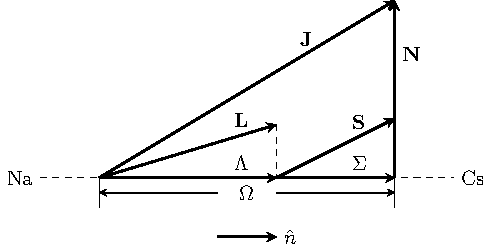
\includegraphics[width=\textwidth]{figures/pa_hunds_case_a.pdf}
  \caption[Hund's~case~(a)]{
    Angular momentum coupling for \textit{Hund's~case~(a)}.
    $\mathbf{L}$ and $\mathbf{S}$ are coupled to the internuclear axis $\hat n$
    and the sum of the projections $\Omega=\Lambda+\Sigma$ is then
    added with the orthogonal component $\mathbf{N}$ to form $\mathbf{J}$.
    \label{fig:pa:hunds-case-a}}
\end{figure}

This is described by the \textit{Hund's~case~(a)}~\cite[p.~523-626]{bransden_physics_2003}.
Molecular states with large binding energies mostly experience interactions
between the atoms at short range where the electrostatic interaction is very strong.
This couples the two electron spins into a total electron spin
$\mathbf{S}\equiv\mathbf{S}_1+\mathbf{S}_2$ via a very strong effective interaction
of the form $\mathbf{S}_1\cdot\mathbf{S}_2$ which originates
from the resulting symmetry of the electron orbital wavefunction.
Similar to atoms, the nuclear spin interaction is also very week compared to
other energy scales so we can ignore the hyperfine structure and only need to consider
$\mathbf{J}\equiv\mathbf{L}+\mathbf{S}+\mathbf{N}$.

The strong electrostatic interaction also creates an effective coupling
between the $\mathbf{L}$ and $\mathbf{S}$ with the internuclear axis $\hat{n}$
causing $\mathbf{L}$ and $\mathbf{S}$ to process rapidly around $\hat{n}$.
This creates two new conserved quantities $\Lambda$ and $\Sigma$
as the projection of $\mathbf{L}$ and $\mathbf{S}$
along $\hat{n}$ respectively.
The total angular momentum along $\hat{n}$ is therefore $\Omega\equiv\Lambda+\Sigma$
and it is added to the $\mathbf{N}$ which is orthogonal to $\hat{n}$ to form
the total angular momentum $\mathbf{J}$~(Fig.~\ref{fig:pa:hunds-case-a}).

The angular momentum state of the molecule is therefore fully characterized by
$|L,\Lambda,S,\Omega,J\rangle$. $\Lambda$ can be $0,1,\dots,L$, $\Omega$ ranges from
$\abs{\Lambda-S}$ to $\Lambda+S$ and $J\geqslant\Omega$.
The $L$ quantum number is specified by the electronic state and will be discussed
in section~\ref{ch:pa:pes}. The rest of the angular momentum quantum numbers
are represented by the \textit{Hund's~case~(a)} term symbol,
\[ ^{2S+1}\Lambda_\Omega \]
similar to the atomic term symbol $^{2S+1}L_J$.
Just as the use of capital English letters $S,P,D,\dots$ are used to represent
$L=0,1,2,\dots$, capital Greek letters $\Sigma,\Pi,\Delta,\dots$ are used
to denote $\Lambda=0,1,2,\dots$ in the term symbol.
An additional symmetry to consider is the reflection about a plane that includes
the internuclear axis.
For $\Lambda>0$ states, the reflection produces a new state at the same energy
creating the so-called $\Lambda$-doubling. For $\Lambda=0$ states, i.e. $\Sigma$ states,
the reflection produces the same state with a phase of $\pm1$.
This phase is also included in the term symbol to fully specify the symmetry of
a $\Sigma$ states as
\[ ^{2S+1}\Sigma_\Omega^{\pm} \]
Note the $\Sigma$ state here should not be confused with the quantum number $\Sigma$.

From the angular momentum relation in Fig.~\ref{fig:pa:hunds-case-a},
we can also determine the energies of different rotational states.
The nuclear rotational energy is given by,
\[
  E_{rot}=B\langle \mathbf{N}^2 \rangle
\]
where $B$ is the rotational constant of the molecule.
For \textit{Hund's~case~(a)} this is,
\begin{align*}
  E_{rot}=&B\langle \mathbf{J}^2 - \Omega^2 \rangle\\
  =&B\langle \mathbf{J}^2 - \Omega^2 \rangle\\
  =&B\paren{J\paren{J+1}-\Omega^2}
\end{align*}
For the last step, note that $\Omega$ is not an angular momentum vector but a projection.
We can easily see that for a given $\Omega$, we have $J\geqslant\Omega$.
Unlike a rigid rotor where $E_{rot}=BN\paren{N+1}$,
the limit on the $J$ means that the spacing between the rotational levels depend on $\Omega$,
\[2\Omega+2,\ 2\Omega+4,\ 2\Omega+6,\ \dots\]
This allows us to determine the $\Omega$ of the state we are addressing
by measuring the state spacing for the lowest few rotational states.

\subsubsection{Near Threshold Bound States}
\label{ch:pa:structure:near-threshold}

For molecular states with a small binding energy, the interaction between the two atoms is
small compared to the internal coupling in the atoms and
the angular momentum coupling is ``atom like''.
In this limit, the total angular momentum $\mathbf{F}_1$ and $\mathbf{F}_2$
for the individual atoms forms $\mathbf{F}_{\mathrm{atom}}=\mathbf{F}_1+\mathbf{F}_2$
which is then coupled to the nuclear rotation $\mathbf{N}$
to form $\mathbf{F}=\mathbf{F}_{\mathrm{atom}}+\mathbf{N}$.
We will discuss this regime in more detail
when we characterize the weakly bound ground states in chapter~\ref{ch:raman-spectroscopy}.

\subsection{Potential Energy Surface}
\label{ch:pa:pes}

Due to the different angular momentum coupling in different regimes,
there is not a consistent way to label the interaction between the two atoms
at both short and long distance.
Nevertheless, by convention, we use the \textit{Hund's~case~(a)} term symbol
since it more accurately represents the state when the interaction energy dominates.

The Hamiltonian (excluding spin for simplicity\footnote{
  Electron spin is implicitly included,
  however, via the symmetry of the electronic wavefunction.}) is,
\begin{align*}
  H=&H_e+T_n
\end{align*}
where the electronic term $H_e$ and the nuclear kinetic term $T_n$ are given by
\begin{align*}
  H_e=&-\sum_i\frac{\hbar}{2m_e}\mathbf{\nabla}_i^2+\frac{e^2}{4\pi\varepsilon_0}\paren{\sum_{i>j}\frac{1}{\abs{\mathbf{r}_i-\mathbf{r}_j}}-\sum_{A=\Na,\Cs}\sum_i\frac{Z_{A}}{\abs{\mathbf{r}_i-\mathbf{R}_{A}}}+\frac{Z_{\Na}Z_{\Cs}}{\abs{\mathbf{R}_{\Cs}-\mathbf{R}_{\Na}}}}\numberthis{eq:pa:pes:he}\\
  T_n=&-\sum_{A=\Na,\Cs}\frac{\hbar^2}{2m_{A}}\mathbf{\nabla}_{A}^2
\end{align*}
and the sum is over all the electrons in the molecule.

\subsubsection{Born-Oppenheimer Approximation}

The Hamiltonian is solved using the Born-Oppenheimer~(BO) approximation.
Because of the large mass difference between the nuclei and the electrons,
we can assume that the electron motion follows the position of the nuclei
instantaneously so that the motion of the nuclei and the electrons can be treated separately.
Formally, this means that the electron wavefunctions is solved using the
electronic term $H_e$ for a given nuclear position $\mathbf{R}_{\Na}$ and $\mathbf{R}_{\Cs}$.
This results in an effective potential $V_{\mathrm{eff}}\paren{\abs{\mathbf{R}_{\Na}-\mathbf{R}_{\Cs}}}$ called
the potential energy surfaces~(PES) for each electronic states.
The solutions to the approximate Hamiltonians $T_n+V_{\mathrm{eff}}$ provide
the vibrational and rotational states of the molecule.

\subsubsection{Franck-Condon Factor}

In addition to the energy of the molecular bound state,
the solution of the nuclear motion also provides information on the selection rules
and coupling strength of transitions between the states.
For an electronic electric dipole transition between states
$|e_1,v_1,j_1\rangle$ and $|e_2,v_2,j_2\rangle$,
where $e_i$, $v_i$ and $j_i$ denotes electronic, vibrational and angular momentum states,
respectively the Rabi frequency under the BO approximation is,
\begin{align*}
  \Omega=&\langle e_1,v_1,j_1|e\mathbf{r}_e\cdot\mathbf{E}\ue^{\ui\mathbf{k}\cdot\mathbf{r}}|e_2,v_2,j_2\rangle\\
  =&\langle e_1(\mathbf{r})|e\mathbf{r}_e\cdot\mathbf{E}|e_2(\mathbf{r})\rangle\langle v_1,j_1|\ue^{\ui\mathbf{k}\cdot\mathbf{r}}|v_2,j_2\rangle
\end{align*}
where $\mathbf{r}$ and $\mathbf{r}_e$ are the molecule and electron coordinates.
For most of the transitions, we can treat the nuclear coordinate dependent transition dipole
moment $\mathbf{D}\paren{\mathbf{r}}\equiv\langle e_1(\mathbf{r})|e\mathbf{r}_e|e_2(\mathbf{r})\rangle$ as a constant $\mathbf{D}$.
Since the size of the molecular wavefunction is also usually much smaller than
the wavelength of the transition, we can also assume $\ue^{\ui\mathbf{k}\cdot\mathbf{r}}\approx 1$,
so we have,
\begin{align*}
  \Omega=&\mathbf{D}\cdot\mathbf{E}\langle j_1|j_2\rangle\langle v_1|v_2\rangle
\end{align*}
The term $\langle j_1|j_2\rangle$ determines the angular momentum selection rule which is
$\Delta\Lambda=0,\pm1$, $\Delta S=\Delta\Sigma=0$, $\Delta\Omega=0,\pm1$ and $\Delta J=0,\pm1$
for \textit{Hund's~case~(a)}~\cite[p.~14-15]{straughan_spectroscopy_1976}.
The term $\langle v_1|v_2\rangle$ gives the coupling strength between vibrational states\footnote{
  Note that $\langle v_1|v_2\rangle$ does not simplify to orthogonality relation
  when $e_1\neq e_2$ since the vibrational wavefunctions belong to different PES.}.
This is called the Franck-Condon principle and the square of the wavefunction overlap
is defined as the Franck-Condon factor~(FCF),
\begin{align*}
  \mathrm{FCF}\equiv&\abs{\langle v_1|v_2\rangle}^2
\end{align*}
For incoherent transition, the transition rate is proportional to $\Omega^2\propto\mathrm{FCF}$.

\subsubsection{Energy Levels of NaCs}

\begin{figure}
  \centering
  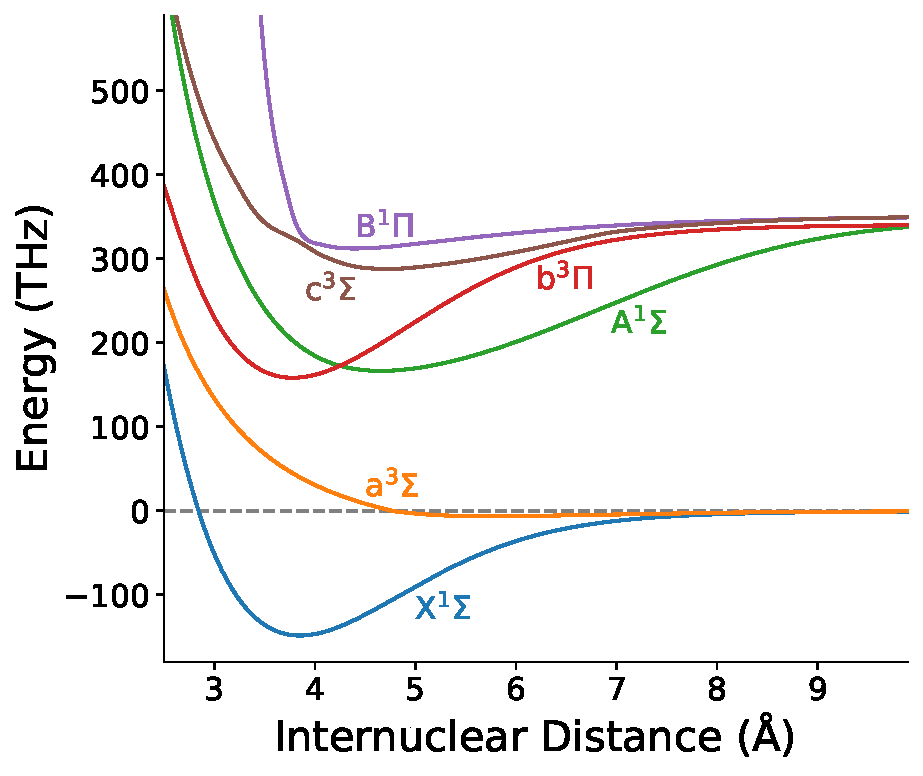
\includegraphics[width=0.9\textwidth]{figures/pa_pes.pdf}
  \caption[NaCs potential energy surfaces]{
    Potential energy surfaces of NaCs with \textit{Hund's~case~(a)} labels.
    Due to spin-orbit coupling, the potentials are not independent of each other.
    The real energy eigenstates of the molecule may be a superposition of multiple
    electronic and spin states.
    \label{fig:pa:pes}}
\end{figure}

Fig.~\ref{fig:pa:pes} shows the relevant PESs for $\mathrm{NaCs}$.
Although the spin-less electronic Hamiltonian~\ref{eq:pa:pes:he} makes it easier
to understand the molecule structure and provides good approximations for the
transition dipole moment and FCF, the absence of spin and the difficulty in exactly solving
a multi-electron system makes it unsuitable to calculate energy levels
for spectroscopy purposes.
Because of this, prediction of the molecular-state energies are calculated using
PESs fitted to experimental data~\cite{docenko_coupling_2006,zaharova_solution_2009,grochola_spin-forbidden_2011,grochola_investigation_2010}.

\section{Photoassociation Spectroscopy}
\label{ch:pa:pa}

\subsection{Beam Path}
\label{ch:pa:beampath}

\begin{figure}
  \centering
  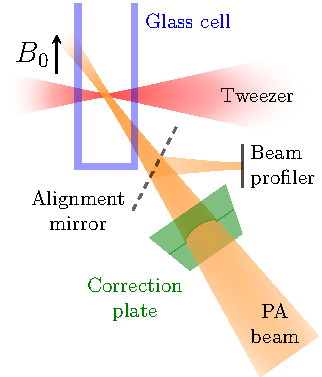
\includegraphics[width=0.7\textwidth]{figures/pa_beampath.pdf}
  \caption[PA beam path]{
    PA beam path including the relative passing with the magnetic field
    the glass vacuum cell and the tweezer.
    In order to compensate for the astigmatism from passing through the glass cell window
    at an angle, we added a correction glass plate into the PA beam path.
    The correction plate has the same thickness and angle of incident with the glass cell window
    but is angled vertically instead of horizontally.
    The alignment mirror and the beam profiler can also be added to the beam path
    in order to measure the chromatic error during alignment.
    \label{fig:pa:beampath}}
\end{figure}

The excited molecular state we would like to address has a bond length of $3\sim8~\text{\AA}$.
The initial atomic state, however, has an average inter-nuclear distance of
$\approx\!1000~\text{\AA}$.
This size mismatch between the wavefunctions of the initial and final state
means the transition typically has a very small FCF~($10^{-10}\sim10^{-8}$).
Because of this, we focus our PA beam onto the tweezer with a beam waist between
$10~\mathrm{\mu m}$ and $30~\mathrm{\mu m}$~(Fig.~\ref{fig:pa:beampath}) in order to
increase the laser intensity and improve the signal contrast.
The tight focus also increases the astigmatism when passing through
the glass cell window at an angle which limits the minimum focus size we can achieve.
Therefore, we added a correction glass plate to fix the astigmatism
in order to minimize the focus size and maximize the beam intensity.

\begin{figure}
  \centering
  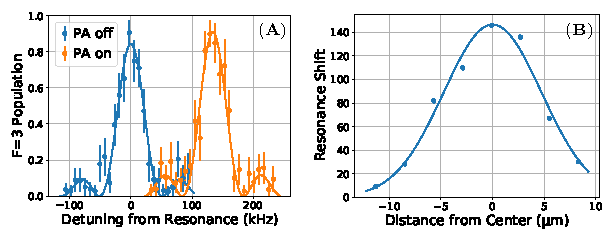
\includegraphics[width=\textwidth]{figures/pa_vectorshift.pdf}
  \caption[PA beam alignment]{
    Measurement of Cs vector light shift from the PA beam for final alignment.
    (A) The effective magnetic field from the circularly polarized PA beam
    causes a shift on the Raman resonance between the $|4,4\rangle$ and $|3,3\rangle$ states.
    (B) Vector light shift as a function of PA beam position
    used to determine the beam center.
    The $1/\ue$ diameter of the beam is measured to be $13.40(72)~\mathrm{\mu m}$.
    \label{fig:pa:alignment}}
\end{figure}

In order to align the PA beam to the tweezer, we use the following alignment procedure,
\begin{enumerate}
\item Light resonant with the Cs atomic transition is sent into the PA beam path.
  This allows us to do the alignment using the procedure we used to align the
  atomic Raman sideband cooling beams as described in section~\ref{ch:rsc:alignment}.
  However, unlike the alignment for the atomic Raman beams,
  due to the larger frequency difference between the PA transition and the Cs atomic
  transition as well as the smaller beam size,
  we cannot use the alignment result from this step directly for the PA beam
  due to the chromatic aberration from the optics in the PA beam path.
\item In order to translate the alignment result from resonance Cs light to that of the PA light,
  we insert a mirror to reflect the PA beam after the last optics in the beam path
  and place a beam profiler at the equivalent location of
  the tweezer~(Fig.~\ref{fig:pa:beampath}).
  This allows us to directly measure location of the focal point for the two wavelengths
  and correct for the chromatic aberration by shifting the focus from the PA light
  to the original focus position from the resonant Cs light.
\item As the final alignment step and to correct for the chromatic aberration of the
  glass window that was not corrected for in the last step,
  we align the PA beam to the atom using signal directly from the atom.
  Due to the large detuning, the scattering rate from the PA beams
  is too low to be used for alignment.
  However, when the PA beam is set to circular polarization, it creates an effective
  magnetic field parallel to the beam propagation direction
  of the form~\cite{thompson_coherence_2013},
  \[ B_{\mathrm{eff}}=-U_0\frac{\delta_2-\delta_1}{\delta_2+2\delta_1}\mathbf{C} \]
  where $U_0$ is the scalar light shift, $\delta_1$ and $\delta_2$ are the detuning from the
  $\mathrm{D}_1$ and $\mathrm{D}_2$ line respectively,
  $\mathbf{\varepsilon}$ is the polarization vector and
  \[\mathbf{C}\equiv\Im\paren{\mathbf{\varepsilon}\times\mathbf{\varepsilon}^*}
    \numberthis{eq:pa:beampath:def-c}\]
  qualifies the ellipticity of the polarization with
  $\abs{C}=1$ for pure circular polarization and $\abs{C}=0$ for linear polarization.
  This effective magnetic field causes a relative shift between the $|4,4\rangle$
  and the $|3,3\rangle$ states which can be measured using
  a Raman transition~(Fig.~\ref{fig:pa:alignment}A).
  By measuring the shift as a function of the beam position,
  we can determine the size and the center of the PA beam and align the beam to
  the atom~(Fig.~\ref{fig:pa:alignment}B).
\end{enumerate}

\subsection{Experiment Sequence and Resonance Frequencies}
\label{ch:pa:sequence-res}

\begin{table}
  \centering
  \caption[PA resonance prediction]{
    Prediction of $|\mathrm{Na(2, 2),Cs(4, 4)}\rangle$ PA resonance frequency
    based on Dunham expansion~\cite{grochola_spin-forbidden_2011,dunham_energy_1932}.
    \label{table:pa:theory-prediction}}
  \begin{tabular}{|c|c|c|c|c|}
    \hline
    Vibrational State&$v'=0$&$v'=12$&$v'=13$&$v'=14$\\\hline
    Resonance Prediction (GHz)&$288722$&$306491$&$307876$&$309252$\\\hline
  \end{tabular}
\end{table}

For the PA spectroscopy, we mainly focus on states with large binding energies
which are expected to be good candidates as the intermediate state
for Raman transfer~(section~\ref{ch:raman-transfer:raman}).
In particular, we scanned the PA light frequency around the $v'=0$ and $v'=12-14$
vibrational states in the $\mathrm{c^3\Sigma}_{\Omega=1}$ potential.
Table~\ref{table:pa:theory-prediction} shows the predicted resonance frequencies
for the PA resonance from $|\mathrm{Na(2, 2),Cs(4, 4)}\rangle$
based on fitting to previous measurements~\cite{grochola_spin-forbidden_2011}.
The frequencies are calculated from a Dunham expansion~\cite{dunham_energy_1932}
that is corrected for the hyperfine structure for the atoms.

In order to observe PA, we first prepare both the Na and Cs atoms in the motional ground states
in the same tweezer~\cite{liu_building_2018}.
We then turn on the PA beam for a set time
followed by separating the atoms into their respective tweezers and imaging the atoms.
When we hit a PA resonance, the excited molecular state will typically decay down
to either a molecular ground state,
which will remain in at most one of the tweezers after the separation,
or an atomic state with high relative motional energy and escape the trap.
In either case, this leads to at least one empty tweezer after the separation.
By measuring the probability of having both the Na and Cs atoms after the PA pulse
conditioned on both atoms being initially loaded,
we can capture the probability of PA event and locate the resonances.

The initial atomic state we used is $|\mathrm{Na(2, 2),Cs(4, 4)}\rangle$
which has $L=0$ and $S=1$.
For atoms in the motional ground state we also have $N=0$ and therefore $J=1$
which should be coupled to $J=0,1,2$ excited states base on the $\Delta J=0,\pm1$ selection rule.
However, since the cooling is not perfect,
we expect some atoms to be initially in the $N=1$ state which can allow a weaker
transition to the $J=3$ states.
Moreover, since the PA beam polarization is circular
and has maximum overlap with the $\sigma^+$ polarization,
the $J=2$ excited state is expected to have the strongest coupling.

\todo{State B field}

\begin{figure}
  \centering
  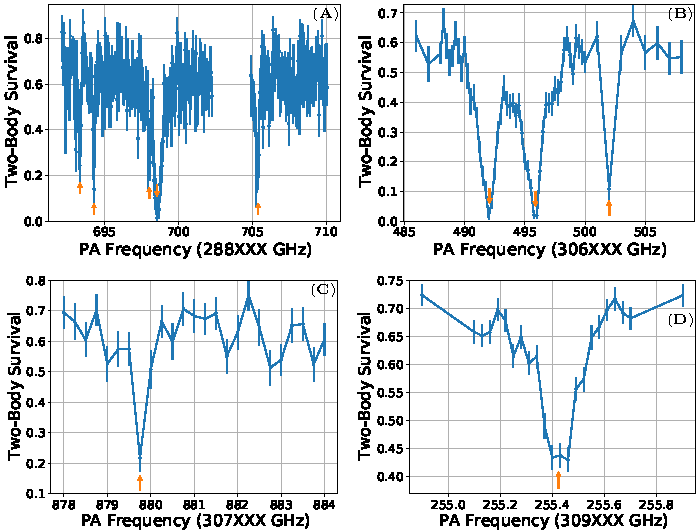
\includegraphics[width=\textwidth]{figures/pa_spectrum.pdf}
  \caption[PA spectrum]{
    PA spectrum for (A) $v'=0$, (B) $v'=12$, (C) $v'=13$, (D) $v'=14$.
    The PA frequency is shown in GHz with an offset.
    Multiple rotational states can be observed for $v'=0$ and $v'=12$.
    $v'=0$ also shows multiple peaks that correspond to
    the hyperfine structure of the molecule.
    The $v'=13$ and $v'=14$ transitions are relatively weak
    and as a result only the strongest line in each transition is measured.
    \label{fig:pa:spectrum}}
\end{figure}

\begin{table}
  \centering
  \caption[PA resonance frequencies]{
    PA resonance frequencies for $v'=0,12-14$.
    The $J$ numbers for $v'=0$ and $v'=12$ are assigned based on the rotational state spacing.
    For $v'=13$ and $v'=14$, we assume the observed line is $J=2$
    which is expected to have the strongest coupling.
    \label{table:pa:all-lines}}
  \begin{tabular}{|c|c|c|c|c|c|}
    \hline
    \multicolumn{2}{|c|}{Vibrational State}&$v'=0$&$v'=12$&$v'=13$&$v'=14$\\\hline
    \multirowcell{5}{Resonance\\(GHz)}&\multirowcell{2}{$J=1$}&$288693.3$&$306492.1$&-&-\\\cline{3-6}
    {}&&$288694.3$&-&-&-\\\cline{2-6}
    {}&\multirowcell{2}{$J=2$}&$288698.0$&$306495.9$&$307879.8$&$309255.4$\\\cline{3-6}
    {}&&$288698.5$&-&-&-\\\cline{2-6}
    {}&$J=3$&$288705.4$&$306502.0$&-&-\\\hline
  \end{tabular}
\end{table}

Fig.~\ref{fig:pa:spectrum} shows the PA spectra measured for different vibrational states
with the frequencies summarized in table~\ref{table:pa:all-lines}.
The spectra for $v'=0$ and $v'=12$ shows three rotational states
whereas only the strongest rotational state is measured for $v'=13$ and $v'=14$.
The $v'=0$ spectrum also shows the hyperfine structure for the lowest two rotational states.

The rotational states of the molecule can be determined from the energy gap between the states
based on the discussion in section~\ref{ch:pa:angular-momenta:deep}.
The ratio of the spacing between the lowest $J$ states we measured are
$1.64$ and $1.61$ for $v'=0$ \footnote{The energy of the strongest hyperfine line is used}
and $v'=12$ respectively.
This is very closed to the ratio of $3/2$ for $\Omega=1$ states.
The main source of the deviation is likely the hyperfine structure
that was ignored in the discussion above.

\subsection{Linewidth}
\label{ch:pa:linewidth}

In addition to the energy, another property of the excited state
that is important for driving a two-photon transition using the state is the linewidth.
This determines the scattering or decoherence rate of
the two-photon transition which then determines
the transfer efficiency~(chapter~\ref{ch:raman-transfer}).
The linewidth, or decay rate, due to electric dipole transitions
is~\cite[p.~197]{bransden_physics_2003},
\begin{align*}
  \Gamma=&\sum_{i}\frac{\omega_i^3d_i^2\mathrm{FCF}_i}{3\pi\varepsilon_0\hbar c^3}
\end{align*}
where $\omega_i$ is the decay frequency, $d_i$ is the transition dipole moment,
and the sum is over all the decay channels.
Since the size of the excited-state electron wavefunction is similar to
that of an unbound excited atomic state pair,
the molecule has a similar transition dipole moment as the corresponding atomic transition
$d_i\approx d_\Cs$. Moreover, since $\sum_i\mathrm{FCF}_i=1$ and $\omega_i\approx\omega_\Cs$
we have
\begin{align*}
  \Gamma\approx&\frac{\omega_\Cs^3d_\Cs^2}{3\pi\varepsilon_0\hbar c^3}\\
  =&\Gamma_\Cs\approx2\pi\times5~\mathrm{MHz}
\end{align*}
Since the PA laser is locked using a wavemeter with a precision
$\approx\!20~\mathrm{MHz}$, we expect the PA linewidth we measured to be limited
by our frequency resolution.

\begin{figure}
  \centering
  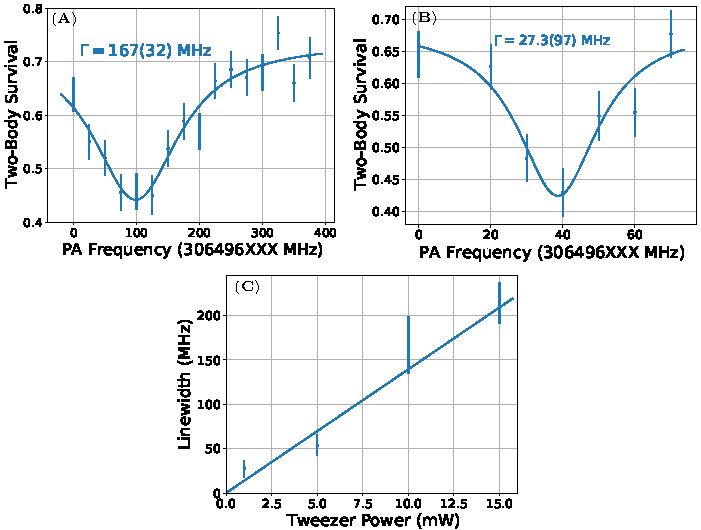
\includegraphics[width=\textwidth]{figures/pa_linewidth_red_twr.pdf}
  \caption[PA linewidth for red detuned tweezer]{
    Fitting of PA linewidth for (A) $10~\mathrm{mW}$, (B) $1~\mathrm{mW}$ tweezer power,
    showing a broad linewidth and a significant difference between the two.
    (C) Fitting of the PA linewidth as a function of tweezer power suggests
    a proportional relation between the two.
    \label{fig:pa:linewidth:red-twr}}
\end{figure}

This is, however, not what is observed in the experiment.
Fig.~\ref{fig:pa:linewidth:red-twr}A shows the narrowest spectrum of the $v'=12, J=2$ PA line
we measured when the tweezer frequency is set to $306344.5~\mathrm{GHz}$
with $10~\mathrm{mW}$ of power. The linewidth is determined to be $167(32)~\mathrm{MHz}$
which is much greater than the theory prediction.
Furthermore, the observed linewidth appears to be dependent on the tweezer power.
The same PA line measured with $1~\mathrm{mW}$ tweezer power
is shown in Fig.~\ref{fig:pa:linewidth:red-twr}B with a significantly narrower linewidth
of $27.3(97)~\mathrm{MHz}$.
In fact, the linewidth appears to be proportional to the tweezer power
as shown in Fig.~\ref{fig:pa:linewidth:red-twr}C,
which suggests that the linewidth may be broadened by a two-photon process.

\begin{figure}
  \centering
  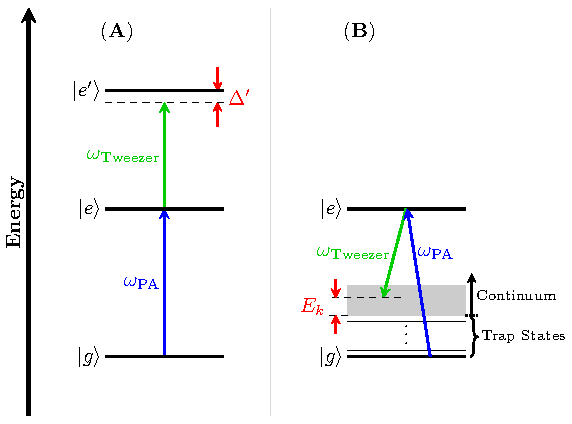
\includegraphics[width=0.939\textwidth]{figures/pa_two_photon_up_vs_down.pdf}
  \caption[Two-photon broadening mechanism for PA.]{
    Potential two-photon broadening mechanism for PA by coupling the excited state $|e\rangle$
    via the tweezer to (A) a higher excited state $|e'\rangle$ or
    (B) the atomic motional continuum.
    (A) For coupling to a higher excited state,
    the broadening depends on the two-photon detuning $\Delta'$ from $|e'\rangle$.
    (B) For coupling to the atomic motional continuum,
    the broadening is a function of the kinetic energy $E_k$ of the atomic state.
    \label{fig:pa:linewidth:up-vs-down}}
\end{figure}

We initially suspected that the source of this broadening is due to the tweezer light
coupling the excited molecular state to another state at
a higher energy~(Fig.~\ref{fig:pa:linewidth:up-vs-down}A).
If this is the case, we would expect the broadening to be a function of
the sum of the tweezer and PA light frequency depending on the detuning from the nearest
two-photon excited state.
However, the broadening does not change significantly when the tweezer frequency
is changed by $\approx\!10~\mathrm{GHz}$ and
is also observed for other excited states including $v'=0$ and $v'=14$
which have very different resonance frequencies.
It is therefore unlikely that this is the broadening mechanism we observe.
Instead, we believe the effect is caused by a $\Lambda$ type two-photon process
coupling the excited state to the atomic ground states.
This mechanism was suggested to us by Olivier Dulieu.
In the following section, I will provide an estimation for such a broadening process.

\subsubsection{Two-Photon Coupling to the Atomic Motional Continuum}
\label{ch:pa:linewidth:two-photn-down}
The broadening of the PA line requires the coupling of the excited state to a continuum of states.
For the ground atomic state, since the state is stable with respect to radiative decay,
this continuum cannot be the photon continuum.
Instead, the excited state is coupled to the relative motional continuum of the atoms.
Physically, this corresponds to a photodissociation process
whereby the atoms fly away with high kinetic energies corresponding
to the detuning of the tweezer~(Fig.~\ref{fig:pa:linewidth:up-vs-down}B).

The photodissociation rate is determined by Fermi's golden rule,
\[
  \Gamma=2\pi\Omega_{if}^2\ \rho_f
\]
where $\Omega_{if}$ is the matrix element between the initial and final state
and $\rho_f$ is the density of states near the final state.
We calculate this by first discretizing the continuum and the rate becomes
\[
  \Gamma=2\pi\frac{{\Omega'_{if}}^2}{\delta}
\]
where $\Omega'_{if}$ is the Rabi frequency between the initial and final state
and $\delta$ is the spacing between the discretized final states.
\todo{Add plot to clarify i, f, Omega_if, Omega_0, etc.}

The Rabi frequency $\Omega'_{if}$ is proportional to the square root of FCF,
which we can calculate for the atomic ground motional states by exact diagonalization
of the atomic wavefunction.
However, due to the high energy~($>\!10~\mathrm{GHz}$) of the final state,
calculating FCF for the target state using this method requires an unrealistic number of
states to be included.
Instead, we approximate it using the results for the atomic ground state
by assuming the FCF to be proportional to the probability density of the non-interacting
atomic wavefunction at zero relative distance so that,
\[
  \Omega'_{if}=\Omega_0\frac{\psi_f\paren{r_{rel}=0}}{\psi_0\paren{r_{rel}=0}}
\]
where $\Omega_0$ is the Rabi frequency between the excited state and
the atomic motional ground state and $\psi_f$ and $\psi_0$ are the
wavefunctions of the final and ground motional atomic state without the molecular potential.
This approximation is justified because,
\begin{enumerate}
\item The molecular potential is short ranged and the excited molecular state is small.
\item Only the final atomic wavefunction within the molecular potential contributes to the FCF.
  For relatively low motional energy
  this wavefunction is proportional to the value of the wavefunction at
  the edge of the molecular potential which is well approximated by
  the atomic wavefunction without the molecular potential.
\end{enumerate}
This approximation remains valid until the de Broglie wavelength for the atomic state
is comparable to the size of the molecular potential which corresponds to
a motional energy of $\approx\!40~\mathrm{GHz}$
and even then the result can still be used as an order of magnitude estimation
for higher motional energies.

For atomic motional ground state, we have,
\begin{align*}
  \psi_0\paren{r_{rel}=0}=&\prod_{i=1}^{3}\paren{\frac{\mu\omega_i}{\pi}}^{1/4}\\
  =&\paren{\frac{\mu^3\omega_1\omega_2\omega_3}{\pi^3}}^{1/4}
\end{align*}
where $\mu$ is the reduced mass $\mu\equiv m_\Na m_\Cs/\paren{m_\Na+m_\Cs}$,
and $\omega_i$'s are the relative trapping frequencies along the three trap axes.
We discretize the continuum state by adding an infinitely deep spherical potential well
of radius $R$ around the center. The radial wavefunctions of the eigenstates
within the well with quantum number $n=1,2,\dots$ is,
\begin{align*}
  \psi_n=&\frac{1}{\sqrt{4\pi}r_{rel}}\sqrt{\frac{2}{R}}\sin\paren{\frac{\pi nr_{rel}}{R}}
\end{align*}
and the corresponding energy,
\begin{align*}
  E_n=&\frac{\pi^2n^2}{2\mu R^2}
\end{align*}
The energy gap between neighboring states is
\begin{align*}
  \delta_n\approx&\frac{\pi^2n}{\mu R^2}
\end{align*}
and the wavefunction value at $r_{rel}=0$ is,
\begin{align*}
  \psi_n\paren{r_{rel}=0}=&\sqrt{\frac{1}{2\pi R}}\left.\frac{\ud}{\ud r_{rel}}\sin\paren{\frac{\pi nr_{rel}}{R}}\right|_{r_{rel}=0}\\
  =&\frac{\pi n}{\sqrt{2\pi R}R}
\end{align*}
Substituting into $\Gamma$ and taking the limit of $R\rightarrow\infty$ we have
\begin{align*}
  \Gamma=&2\pi\frac{\Omega_0^2}{\delta}\frac{\psi_f^2\paren{r_{rel}=0}}{\psi_0^2\paren{r_{rel}=0}}\\
  =&2\pi\Omega_0^2\frac{\mu R^2}{\pi^2n}\frac{\pi^2 n^2}{2\pi R^3}\sqrt{\frac{\pi^3}{\mu^3\omega_1\omega_2\omega_3}}\\
  =&\Omega_0^2\frac{n}{R}\sqrt{\frac{\pi^3}{\mu\omega_1\omega_2\omega_3}}\\
  =&\Omega_0^2\sqrt{\frac{2\pi E}{\omega_1\omega_2\omega_3}}
     \numberthis{eq:pa:linewidth:two-photn-down:rates}
\end{align*}
For the condition in Fig.~\ref{fig:pa:linewidth:red-twr}A
we have $\Omega_0\approx2\pi\times1~\mathrm{MHz}$\footnote{From theory prediction},
$E=2\pi\times151~\mathrm{GHz}$ and $\omega_{1,2,3}=2\pi\times\{20,100,100\}~\mathrm{kHz}$
which predicts a broadened linewidth of $\Gamma=2\pi\times70~\mathrm{GHz}$.
This prediction is only an estimate due to the breakdown of the approximation
for the coupling strength we used and is in fact much broader than the observed value.
Nevertheless, it confirms that this broadening mechanism can indeed cause
a significant broadening comparable to the observed linewidth.

\subsubsection{Eliminating the Broadening with Blue Detuned Tweezer}
\label{ch:pa:linewidth:blue-tweezer}
\begin{figure}
  \centering
  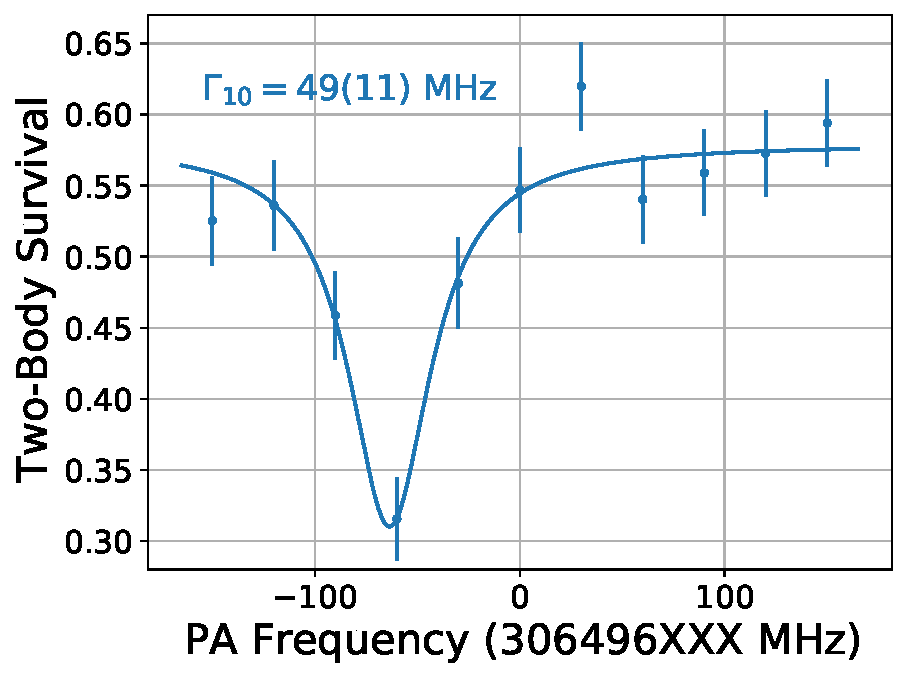
\includegraphics[width=0.55\textwidth]{figures/pa_spectrum_v12_blue_10.pdf}
  \caption[PA linewidth for blue detuned tweezer]{
    Fitting of PA linewidth for $10~\mathrm{mW}$ tweezer power at $306612~\mathrm{GHz}$.
    The linewidth is significantly narrower than the value measured when the tweezer
    is red detuned from the PA resonance~(Fig.~\ref{fig:pa:linewidth:red-twr}).
    \label{fig:pa:linewidth:blue-twr}}
\end{figure}
Another prediction from the theory is that if the tweezer light is blue detuned from
the PA line, the two-photon process will not couple to the motional continuum anymore
and there should be no broadening of the line\footnote{
  Note that the tweezer is still red detuned from the atomic state which
  provides most of the trapping potential}.
We can confirm this by measuring the linewidth of the same PA line with the tweezer
frequency set to $306612~\mathrm{GHz}$,
which is $121~\mathrm{GHz}$ blue detuned from the PA resonance.
The result shown in Fig.~\ref{fig:pa:linewidth:blue-twr}
confirms that the linewidth is indeed narrower for this tweezer frequency.

\subsubsection{Implication on Two-Photon Transition to Ground Molecular States}
\label{ch:pa:linewidth:raman}

\begin{figure}
  \centering
  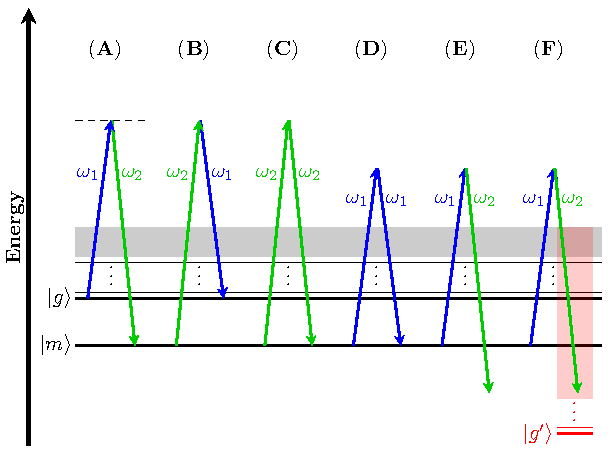
\includegraphics[width=\textwidth]{figures/pa_two_photon_down_raman.pdf}
  \caption[Two-photon transition from molecular state.]{
    Effect of two-photon coupling to atomic continuum on molecular state.
    (A) Raman transition from the atomic ground state $|g\rangle$
    to the molecular bound state $|m\rangle$ using two Raman beams with frequencies
    $\omega_1$ and $\omega_2$.
    (B-E) Two photon transitions starting from the molecular state $|m\rangle$
    with different frequency combinations without additional atomic spin states.
    (B) This is the reverse Raman transition and reaches the initial atomic state.
    (C,D) The frequency pairs couples back to $|m\rangle$.
    (E) This couples to an energy below $|m\rangle$.
    Note that none of the two-photon transitions from $|m\rangle$ in (B-E) ends up in
    the atomic motional continuum and therefore unaffected by the broadening mechanism
    discussed in this section.
    (F) The present of another atomic spin state $|g'\rangle$ with lower energy
    allows the two-photon transition from $|m\rangle$ to be coupled to the
    motional continuum corresponding to the new spin state.
    Note that only the frequency combination similar to (E) is shown for simplicity.
    Coupling channel corresponding to (B-D) also exists which could allow coupling
    to the same continuum at different motional energies.
    \label{fig:pa:linewidth:two-photon-down-raman}}
\end{figure}

Since the broadening is caused by two-photon coupling to high energy atomic motional states,
the observed linewidth in a PA measurement cannot be directly translated to
the scattering rate during a two-photon transition that uses a different set of laser frequencies.

In fact, with a single ground atomic spin state, the scattering rate for the final molecular
state during a two-photon transition is not affected by this effect.
As shown in Fig.~\ref{fig:pa:linewidth:two-photon-down-raman}B-E,
the molecular state cannot reach the atomic motional continuum via a two-photon transition.
The atomic state, on the other hand, can reach the continuum though the loss rate is in general
much lower than the molecular state
and is usually not the limiting factor for the transfer efficiency.

The molecular state can also couple to a different motional continuum if there are other
atomic spin states with lower energies~(Fig.~\ref{fig:pa:linewidth:two-photon-down-raman}F).
Since the stable atomic state has the lowest energy among all the ones with the same total $m_F$,
such a state must have a different total $m_F$ than the initial state.
Therefore, such coupling is forbidden if the two Raman beams both have $\pi$ polarization,
as is the case for the Raman transition in chapter~\ref{ch:raman-spectroscopy}
and \ref{ch:raman-transfer}, and will not cause any loss due to this mechanism.
Polarization impurity, however, can allow such coupling and enable this loss process.

\section{Summary and Outlook}
\label{ch:pa:summary}
We continued our study of the interaction between two atoms in the optical tweezer.
We characterized the excited molecular potential by measuring
the energy of bound states using photoassociation spectroscopy
and identified the states based on their rotational structure.
On the other hand, the high intensity of the optical tweezer
also creates unique challenges that can lead to dissociation or loss of the atoms or molecules.
We studied one of the effects and confirmed our model for the loss process with
additional measurements and discussed its implication for future experiments.
The identification of the excited molecular state opens up the pathway
to the formation of a single ground-state molecule via two-photon process
and will be the focus of later chapters.
